\section{Modelle}

\begin{frame}{Modelle in der Wissenschaft}
\begin{block}{Remark}
Sample text
\end{block}

\begin{alertblock}{Important theorem}
Sample text in red box
\end{alertblock}

\begin{examples}
Sample text in green box. The title of the block is ``Examples".
\end{examples}
    
\end{frame}


\begin{frame}{Lists}
  \begin{columns}[T,onlytextwidth]
    \column{0.33\textwidth}
      Items
      \begin{itemize}
        \item Milk \item Eggs \item Potatos
      \end{itemize}

    \column{0.33\textwidth}
      Enumerations
      \begin{enumerate}
        \item First, \item Second and \item Last.
      \end{enumerate}

    \column{0.33\textwidth}
      Descriptions
      \begin{description}
        \item[PowerPoint] Meeh. \item[Beamer] Yeeeha.
      \end{description}
  \end{columns}
\end{frame}

\begin{frame}{Modelle in der Wissenschaft}
    \begin{quote}
        In den Wissenschaften werden Modelle aus den unterschiedlichsten Gründen zur Originalrepräsentation herangezogen.~\parencite[138]{stachowiak}
    \end{quote}
    % ----------------------------------------------
  \begin{columns}[T,onlytextwidth]
  \metroset{block=fill}
    \column{0.3\textwidth}
      \begin{block}{Default}
            \begin{quote}
        In den Wissenschaften werden Modelle aus den unterschiedlichsten Gründen zur Originalrepräsentation herangezogen.~\parencite[138]{stachowiak}
    \end{quote}
      \end{block}

      \begin{alertblock}{Alert}
        Block content.
      \end{alertblock}

      \begin{exampleblock}{Example}
        Block content.
      \end{exampleblock}
    % ----------------------------------------------
    \column{0.3\textwidth}

      \metroset{block=fill}

      \begin{block}{Default}
        Block content.
      \end{block}

      \begin{alertblock}{Alert}
        Block content.
      \end{alertblock}

      \begin{exampleblock}{Example}
        Block content.
      \end{exampleblock}
      
    % ----------------------------------------------
    \column{0.3\textwidth}

      \metroset{block=fill}

      \begin{block}{Default}
        Block content.
      \end{block}

      \begin{alertblock}{Alert}
        Block content.
      \end{alertblock}

      \begin{exampleblock}{Example}
        Block content.
      \end{exampleblock}
  \end{columns}
\end{frame}


\section{Blocks Columns}
\begin{frame}{Blocks}
  Three different block environments are pre-defined and may be styled with an
  optional background color.

  \begin{columns}[T,onlytextwidth]
    \column{0.5\textwidth}
      \begin{block}{Default}
        Block content.
      \end{block}

      \begin{alertblock}{Alert}
        Block content.
      \end{alertblock}

      \begin{exampleblock}{Example}
        Block content.
      \end{exampleblock}

    \column{0.5\textwidth}

      \metroset{block=fill}

      \begin{block}{Default}
        Block content.
      \end{block}

      \begin{alertblock}{Alert}
        Block content.
      \end{alertblock}

      \begin{exampleblock}{Example}
        Block content.
      \end{exampleblock}

  \end{columns}
\end{frame}

\section{SQL-CodeSlides}
\begin{frame}[fragile]{SQL}
just minted sql
\begin{minted}{sql}
SELECT DISTINCT column_list
FROM table_list
    JOIN table ON join_condition
WHERE row_filter
ORDER BY column
LIMIT count OFFSET offset
GROUP BY column
HAVING group_filter;
\end{minted}
\end{frame}


\begin{frame}[fragile]{Test}
sqlcode  

\begin{sqlcode}
SELECT DISTINCT column_list
FROM table_list
    JOIN table ON join_condition
WHERE row_filter
ORDER BY column
LIMIT count OFFSET offset
GROUP BY column
HAVING group_filter;
\end{sqlcode}

\end{frame}


\begin{frame}[fragile]{Test}
htmlcode  

\begin{htmlcode}
<html>
<head>
<meta http-equiv="Content-Type" 
   content="text/html; charset=UTF-8">
<meta http-equiv="Content-Language" 
\end{htmlcode}

\end{frame}

%------------------------------------------------------------------------------
\begin{frame}[fragile]{Blocks}
TEST
  \begin{columns}[T,onlytextwidth]
    \column{0.5\textwidth}
      \begin{itemize}
          \item info
      \end{itemize}
      
      \begin{block}{Default}
        Block content.
      \end{block}

      \begin{alertblock}{Alert}
        Block content.
      \end{alertblock}

      \begin{exampleblock}{Example}
        Block content.
      \end{exampleblock}

    \column{0.5\textwidth}
      \begin{greysql}
SELECT DISTINCT column_list
FROM table_list
    JOIN table ON join_condition
WHERE row_filter
ORDER BY column
LIMIT count OFFSET offset
GROUP BY column
HAVING group_filter;
\end{greysql}

  \end{columns}
\end{frame}

%------------------------------------------------------------------------------
\begin{frame}[fragile]{Blocks}
  Three different block environments are pre-defined and may be styled with an
  optional background color.

  \begin{columns}[T,onlytextwidth]
    \column{0.4\textwidth}
      \begin{itemize}
          \item info
      \end{itemize}
      
      \begin{block}{Default}
        Block content.
      \end{block}

      \begin{alertblock}{Alert}
        Block content.
      \end{alertblock}

      \begin{exampleblock}{Example}
        Block content.
      \end{exampleblock}

    \column{0.6\textwidth}
\begin{sqlcode}
SELECT DISTINCT column_list
FROM table_list
    JOIN table ON join_condition
WHERE row_filter
ORDER BY column
LIMIT count OFFSET offset
GROUP BY column
HAVING group_filter;
\end{sqlcode}

  \end{columns}
\end{frame}

\section{Modelle nochmal}
%------------------------------------------------------------------------------
\begin{frame}{Modelle in der Wissenschaft}
    \begin{quote}
        In den Wissenschaften werden Modelle aus den unterschiedlichsten Gründen zur Originalrepräsentation herangezogen.~\parencite[138]{stachowiak}
    \end{quote}
    \begin{quote}
        Als Demonstrationsmodelle werden sie zur
Veranschaulichung von (weniger anschaulichen oder
unanschaulichen) Zusammenhängen benutzt, \punkti.~\parencite[138]{stachowiak}
    \end{quote}
    % ----------------------------------------------
  \begin{columns}[T,onlytextwidth]
  %\metroset{block=fill}
    \column{0.5\textwidth}
      \begin{block}{Default}
            \begin{quote}
        In den Wissenschaften werden Modelle aus den unterschiedlichsten Gründen zur Originalrepräsentation herangezogen.~\parencite[138]{stachowiak}
    \end{quote}
      \end{block}

      \begin{alertblock}{Alert}
        Block content.
      \end{alertblock}

      \begin{exampleblock}{Example}
        Block content.
      \end{exampleblock}
    % ----------------------------------------------

    \column{0.5\textwidth}

      \metroset{block=transparent}

      \begin{block}{Demonstrationsmodelle}
            \begin{quote}
        Als Demonstrationsmodelle werden sie zur
Veranschaulichung von (weniger anschaulichen oder
unanschaulichen) Zusammenhängen benutzt, \punkti.~\parencite[138]{stachowiak}
    \end{quote}
      \end{block}

      \begin{alertblock}{Alert}
        Block content.
      \end{alertblock}

      \begin{exampleblock}{Example}
        Block content.
      \end{exampleblock}

  \end{columns}
\end{frame}


%------------------------------------------------------------------------------
\begin{frame}{Modelltheorie Fortsetzung}
Grundlagen der Datenmodellierung
\begin{itemize}\small
    \item Daten
    \item Modellierung 
    \item Modelle
\end{itemize}
\begin{columns}[T,onlytextwidth]
\column{0.45\textwidth}

\metroset{block=fill}
    \begin{block}{\cite[131]{stachowiak}}
        \begin{quote}
        
        \end{quote}
    \end{block}
\begin{exampleblock}{\footnotesize Welche Informationen bzw. welches (abstrakte) Wissen steckt im Globus bzw. in Google Maps/Google Earth? }
    \begin{itemize}\footnotesize
        \item 
    \end{itemize}
\end{exampleblock}
% Aus welchen Gründen bzw. zu welchem Zweck könnten die Modelle zur Originalrepräsentation herangezogen werden?

\column{0.5\textwidth}
\begin{alertblock}{Wozu?}
\begin{enumerate}\small
    \item 
\end{enumerate}
\end{alertblock}

\begin{alertblock}{Wie? (Operationen mit dem Modell)}
\begin{enumerate}\small
    \item 
\end{enumerate}
\end{alertblock}
\end{columns}

\end{frame}


%------------------------------------------------------------------------------
\begin{frame}{Operative Modelle}
  \begin{columns}[T,onlytextwidth]
  \metroset{block=fill}
    \column{0.5\textwidth}
    
    \begin{quote} 
    \end{quote}
    % ----------------------------------------------
    \column{0.5\textwidth}
    \metroset{block=fill}
        \begin{block}{\cite[131]{stachowiak}}
        \begin{quote}
            
        \end{quote}
    \end{block}
    \metroset{block=fill}
      \begin{block}{\footnotesize Modellbildung Bsp. Globus}
      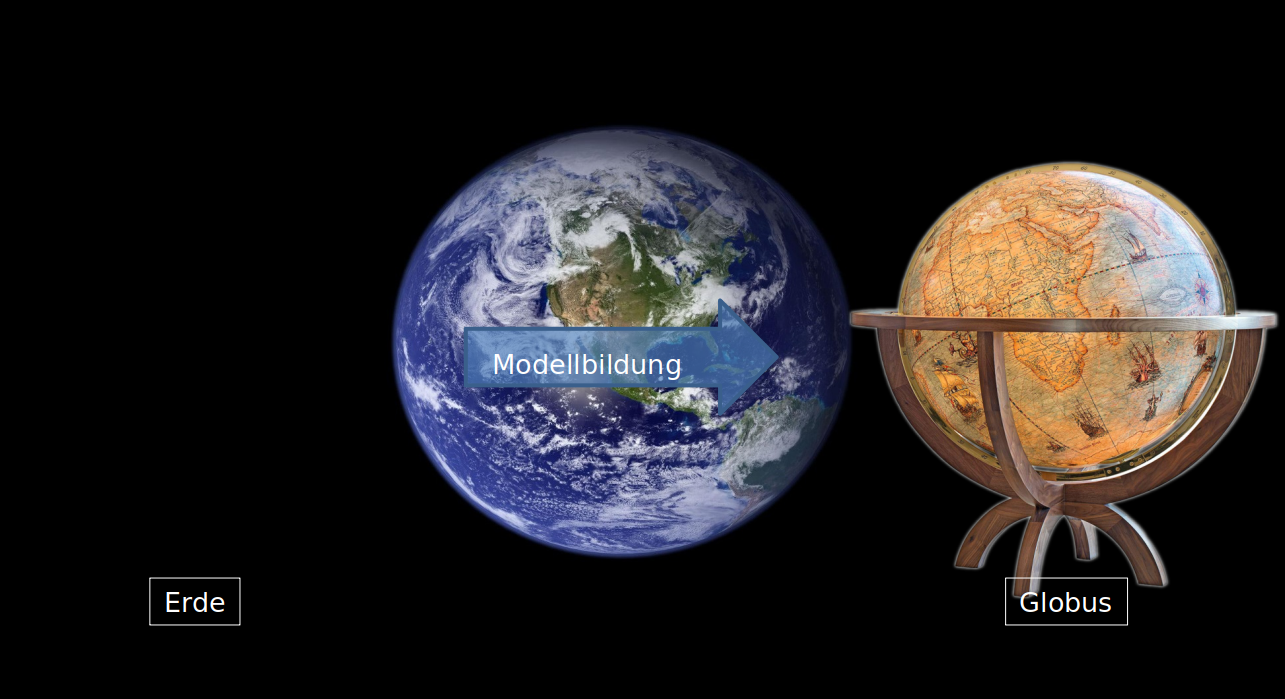
\includegraphics[width=0.95\textwidth]{img/modell-globus2.png}
      \end{block}

  \end{columns}

\begin{columns}[T,onlytextwidth]

\column{0.3\textwidth}

\column{0.3\textwidth}

\column{0.3\textwidth}

\end{columns}
\end{frame}
%------------------------------------------------------------------------------
\begin{frame}{Experimentalmodelle}
    \begin{quote}
„\punkti als Experimentalmodelle dienen sie der Ermittlung
oder Überprüfung von Hypothesen \punkti“~\parencite[139]{stachowiak}
    \end{quote}
    \begin{quote}
        Als Demonstrationsmodelle werden sie zur
Veranschaulichung von (weniger anschaulichen oder
unanschaulichen) Zusammenhängen benutzt, \punkti.~\parencite[138]{stachowiak}
    \end{quote}
    % ----------------------------------------------
  \begin{columns}[T,onlytextwidth]
  \metroset{block=fill}
    \column{0.3\textwidth}
      \begin{block}{Default}
      \href{https://youtu.be/K0aPuLn76H0}{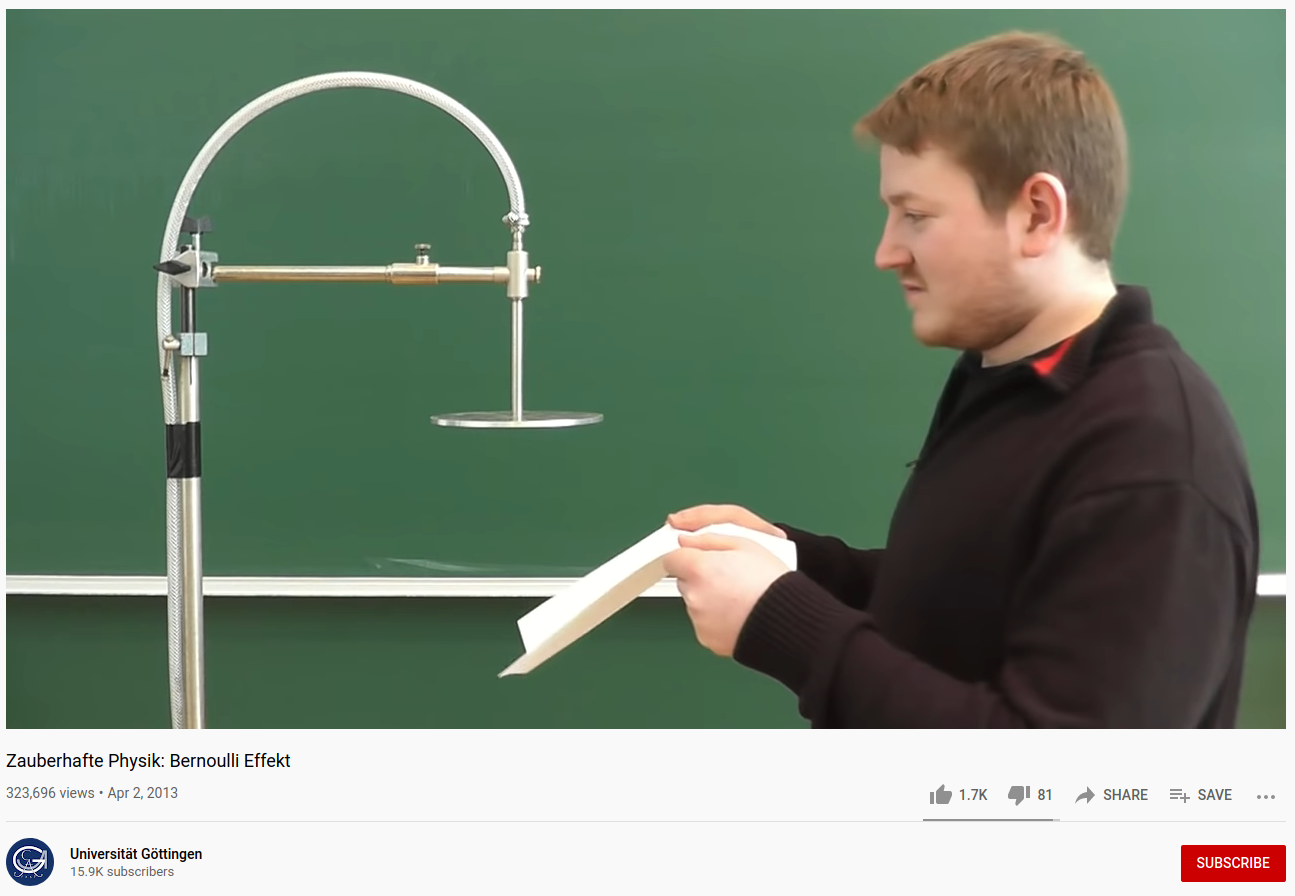
\includegraphics[width=0.3\textwidth]{img/physik-bernoulli.png}}
      \end{block}

      \begin{alertblock}{Alert}
        Block content.
      \end{alertblock}

      \begin{exampleblock}{Example}
        Block content.
      \end{exampleblock}
    % ----------------------------------------------
    \column{0.3\textwidth}

      \metroset{block=fill}

      \begin{block}{Default}
        Block content.
      \end{block}

      \begin{alertblock}{Alert}
        Block content.
      \end{alertblock}

      \begin{exampleblock}{Example}
        Block content.
      \end{exampleblock}
      
    % ----------------------------------------------
    \column{0.3\textwidth}

      \metroset{block=fill}

      \begin{block}{Default}
        Block content.
      \end{block}

      \begin{alertblock}{Alert}
        Block content.
      \end{alertblock}

      \begin{exampleblock}{Example}
        Block content.
      \end{exampleblock}
  \end{columns}
\end{frame}

{\setbeamercolor{palette primary}{fg=black, bg=yellow}
\begin{frame}[standout]
  Questions?
\end{frame}
}

\appendix

\begin{frame}[fragile]{Backup slides}
  Sometimes, it is useful to add slides at the end of your presentation to
  refer to during audience questions.

  The best way to do this is to include the \verb|appendixnumberbeamer|
  package in your preamble and call \verb|\appendix| before your backup slides.

  \themename will automatically turn off slide numbering and progress bars for
  slides in the appendix.
\end{frame}

\begin{frame}[allowframebreaks]{References}

  \bibliography{demo}
  \bibliographystyle{abbrv}

\end{frame}





%------------------------------------------------------------------------------
\begin{frame}[fragile]{Blocks}
  Three different block environments are pre-defined and may be styled with an
  optional background color.

  \begin{columns}[T,onlytextwidth]
    \column{0.4\textwidth}
      \begin{itemize}
          \item info
      \end{itemize}
      
      \begin{block}{Default}
        Block content.
      \end{block}

      \begin{alertblock}{Alert}
        Block content.
      \end{alertblock}

      \begin{exampleblock}{Example}
        Block content.
      \end{exampleblock}

    \column{0.6\textwidth}
\begin{sqlcode}
SELECT DISTINCT column_list
FROM table_list
    JOIN table ON join_condition
WHERE row_filter
ORDER BY column
LIMIT count OFFSET offset
GROUP BY column
HAVING group_filter;
\end{sqlcode}

  \end{columns}
\end{frame}


%------------------------------------------------------------------------------
\begin{frame}[fragile]{Blocks}
  Three different block environments are pre-defined and may be styled with an
  optional background color.

  \begin{columns}[T,onlytextwidth]
    \column{0.5\textwidth}
      \begin{itemize}
          \item info
      \end{itemize}
      
      \begin{block}{Default}
        Block content.
      \end{block}

      \begin{alertblock}{Alert}
        Block content.
      \end{alertblock}

      \begin{exampleblock}{Example}
        Block content.
      \end{exampleblock}

    \column{0.5\textwidth}
      \begin{greysql}
SELECT DISTINCT column_list
FROM table_list
    JOIN table ON join_condition
WHERE row_filter
ORDER BY column
LIMIT count OFFSET offset
GROUP BY column
HAVING group_filter;
\end{greysql}

  \end{columns}
\end{frame}


%------------------------------------------------------------------------------
\begin{frame}{Blocks}
  Three different block environments are pre-defined and may be styled with an
  optional background color.

  \begin{columns}[T,onlytextwidth]
    \column{0.5\textwidth}
      \begin{block}{Default}
        Block content.
      \end{block}

      \begin{alertblock}{Alert}
        Block content.
      \end{alertblock}

      \begin{exampleblock}{Example}
        Block content.
      \end{exampleblock}

    \column{0.5\textwidth}

      \metroset{block=fill}

      \begin{block}{Default}
        Block content.
      \end{block}

      \begin{alertblock}{Alert}
        Block content.
      \end{alertblock}

      \begin{exampleblock}{Example}
        Block content.
      \end{exampleblock}

  \end{columns}
\end{frame}

%------------------------------------------------------------------------------
\begin{frame}[fragile]{Blocks}
TEST
  \begin{columns}[T,onlytextwidth]
    \column{0.5\textwidth}
      \begin{itemize}
          \item info
      \end{itemize}
      
      \begin{block}{Default}
        Block content.
      \end{block}

      \begin{alertblock}{Alert}
        Block content.
      \end{alertblock}

      \begin{exampleblock}{Example}
        Block content.
      \end{exampleblock}

    \column{0.5\textwidth}
      \begin{greysql}
SELECT DISTINCT column_list
FROM table_list
    JOIN table ON join_condition
WHERE row_filter
ORDER BY column
LIMIT count OFFSET offset
GROUP BY column
HAVING group_filter;
\end{greysql}

  \end{columns}
\end{frame}

%------------------------------------------------------------------------------
\begin{frame}[fragile]{Blocks}
  Three different block environments are pre-defined and may be styled with an
  optional background color.

  \begin{columns}[T,onlytextwidth]
    \column{0.4\textwidth}
      \begin{itemize}
          \item info
      \end{itemize}
      
      \begin{block}{Default}
        Block content.
      \end{block}

      \begin{alertblock}{Alert}
        Block content.
      \end{alertblock}

      \begin{exampleblock}{Example}
        Block content.
      \end{exampleblock}

    \column{0.6\textwidth}
\begin{sqlcode}
SELECT DISTINCT column_list
FROM table_list
    JOIN table ON join_condition
WHERE row_filter
ORDER BY column
LIMIT count OFFSET offset
GROUP BY column
HAVING group_filter;
\end{sqlcode}


\begin{columns}
  \column{0.45\textwidth}
  \column{0.55\textwidth}
\end{columns}
  

  \end{columns}
\end{frame}




